\documentclass[11pt,a4paper]{article}
\usepackage{fullpage}
\usepackage[T1]{fontenc}
\usepackage[utf8]{inputenc}
\usepackage{hyperref}
\usepackage{pgf}
\usepackage{tikz}
\usepackage[nottoc, notlof, notlot]{tocbibind}
\usepackage{float}

%\setlength{\parindent}{2em}

\title{\textbf{Ambiruptor}\\The Lexical Ambiguation
    Interruptor\\~\\Mid-term Report}
 \author{Boumediene Brikci Sid\\
         Maria Boritchev\\
         Victor Hublitz\\
         Simon Mauras\\
         Pierre Ohlmann\\
         Ievgeniia Oshurko\\
         Samir Tendjaoui\\
         Thi Xuan Vu}

\begin{document}

\maketitle

\vspace{2cm}
\subsection*{Abstract} 

The main point of our project is to develop a word-sense disambiguation tool. Our aim is to be able, given a certain text, to determine the actual meaning of each ambiguous word. To this end we use Wikipedia, and more specifically its internal links, in order to produce an annotated corpus from which a machine learning framework is developed. At the present time, we are clear about our objectives and we have chosen the abstract design of our future code. Furthermore, the coding part is now well advanced as we achieve mining Wikipedia and have already implemented several feature extractors.

\newpage

\tableofcontents

\newpage

\section{Presentation}

Word Sense Disambiguation is a Natural Language Processing task that lies in the assignment of the appropriate meaning to a word according to a given context, and its separation from other possible meanings. Since the 1940s, this problem has proved its difficulty and the lack of database has forced people to label each word manually.

Nowadays, the Internet creates new possibilities to get sufficiently big databases and the use of new machine-learning methods has given more efficient results on this open problem.    

%\subsection{Word Sense Disambiguation}

\noindent There are several possible applications of Word Sense Disambiguation:
\begin{itemize}
	\item Machine Translation
	\item Information Retrieval
	\item Semantic Parsing
	\item Speech Synthesis and Recognition
\end{itemize}

\subsection{Ambiruptor project}

The main objective of the \textbf{Ambiruptor project} is to produce an efficient tool that gives the correct meaning of ambiguous words in a text. Our tool will be based on several supervised machine learning concepts. We use Wikipedia to build our learning corpus and to annotate it according to its internal links.

\noindent All the code we produce is under the \href{http://www.gnu.org/licenses/gpl-3.0.html}{GNU GPLv3} license.

\subsection{Work team}

Our team consists of 8 master students of the ENS of Lyon: Boumediene Brikci Sid, Maria Boritchev, Victor Hublitz, Simon Mauras, Pierre Ohlmann, Ievgeniia Oshurko, Samir Tendjaoui and Thi Xuan Vu. The coordinators of the project are Simon Mauras and Ievgeniia Oshurko.

\subsection{Work advancement}

\noindent In the project proposal, we presented the project split in several steps:
\begin{itemize}
    \item Research
    \item Design \& Implementation (API)
    \item Test (evaluation of performances)
    \item Integration (plugins \& apps)
\end{itemize}
We are currently working on the implementation part. The decisions made during the research and design parts are listed below.

\newpage

\subsection{Following us}

You can follow us using our website (\url{http://ambiruptor.github.io}) or contact us by email at \url{ambiruptor@ens-lyon.fr}.


\section{Research}

First of all, we checked the state of the art of word-sense disambiguation, data mining and machine learning. Then, we focused on the matching problem of those different modules together to choose the parameters.
 
\subsection{Natural Language Processing}
Word Sense Disambiguation is a Natural Language Processing task for which the context of the considered word is of major importance. In order to process this context one needs to define so-called \textit{features}, that are key points to look for in the input sentence. The disambiguation cannot be done without these. Features that can be considered are part-of-speech labelling, morphological forms identification and frequency considerations (see \cite{features}). 


\subsection{Machine Learning}
In order to solve the Word Sense Disambiguation problem, the following methods are usually considered:
\begin{itemize}
    \item Dictionary-based methods
    \item Unsupervised methods
    \item Supervised methods
\end{itemize}
The supervised learning is currently the most effective method, but it requires an annotated corpus in order to train the algorithm. Our goal is to provide a tool using a supervised learning algorithm on automatically built corpora. The advantage of this approach is that our tool retains the accuracy of supervised methods and can easily be adapted (different languages, ...).

\subsection{Our choice}
There are several approaches to solve the Word Sense Disambiguation problem, many of which achieve good results. We try to choose and to implement several learning models and feature extractors to be able to compare them and to pick the best ones afterwards.

\newpage


\subsubsection{Learning models}

The objective is to associate the right sense to an ambiguous word. We consider two possible solutions: we can either get one single model that gives the correct meaning for every word, or get one model per ambiguous word. The second option is chosen for several reasons:
\begin{itemize}
    \item The computations can be easily distributed.
    \item The feature extraction can be specific to the ambiguous word.
    \item The corpus for each model is smaller.
\end{itemize}

\subsubsection{Features}

Using a learning model accurately requires a lot of experiments; indeed, some features are better than others. In addition to usual features used for natural language processing (part-of-speech labelling), we decided to implement the one introduced in \cite{features}, and also some features we considered important, such as the type of prepositions in the sentence (time, place, etc.).
\\

\begin{table}[H]
    \centering
    \begin{tabular}{|l|l|}
        \hline
        \textbf{Meaning} & \textbf{Related words} \\
        \hline
        Living plant & green, algae, land, water, food, cell, ... \\
        \hline
        Manufacturing plant & factory, industry, manufactory, build, product, \\
        & engine, process, artisan, chemical, ...\\
        \hline
    \end{tabular}
    \caption{Related words for "plant"}
    \label{fig:features}
\end{table}

\noindent If we want to disambiguate one occurrence of the word "plant" in a text, the presence of words related to one of the meanings is a rather good hint.

\subsubsection{Text corpora and data mining}

The supervised learning approach for text disambiguation implies having a corpus with already labelled ambiguous words. We have two choices for getting such a corpus: either by manually labelling ambiguous words or by using existing resources to build our data automatically. The first solution is more accurate but requires much more time, therefore we decided to choose the second one.

Manual use of Wikipedia data for disambiguation has already been done in \cite{wikipedia}. The important point in our work is the fact that no human annotations are required. The main idea is to consider that each meaning of an ambiguous word is represented by a wiki-page. The disambiguation page allows us to get the different meanings of a given word. Links between wiki-pages are considered labelled words. The figure \ref{fig:wikipedia} describes how we build a corpus to disambiguate a word.

\begin{figure}[h!]
    \centering
    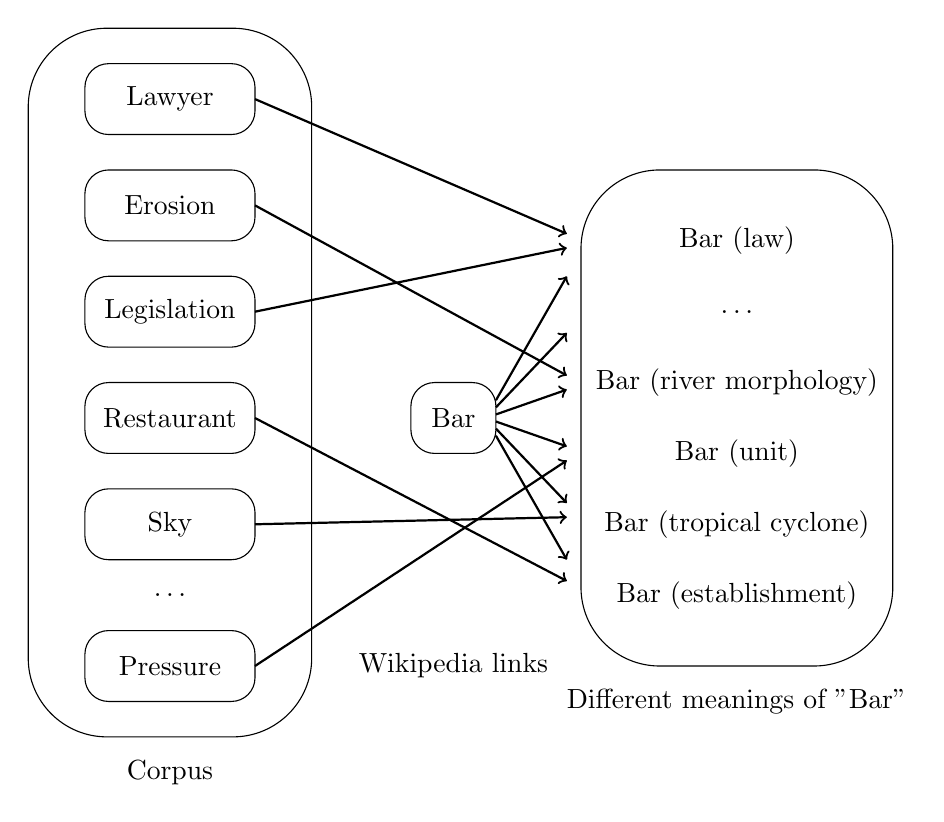
\begin{tikzpicture}[scale=0.9]
        \node at (0, 7) {Lawyer} ;
        \draw [rounded corners=3mm] (-1.2,6.5) rectangle (1.2,7.5) ;
        \draw[thick,->] (1.2,7) -- (5.6,5.1) ;
        
        \node at (0, 5.5) {Erosion} ;
        \draw [rounded corners=3mm] (-1.2,5) rectangle (1.2,6) ;
        \draw[thick,->] (1.2,5.5) -- (5.6,3.1) ;
        
        \node at (0, 4) {Legislation} ;
        \draw [rounded corners=3mm] (-1.2,3.5) rectangle (1.2,4.5) ;
        \draw[thick,->] (1.2,4) -- (5.6,4.9) ;
        
        \node at (0, 2.5) {Restaurant} ;
        \draw [rounded corners=3mm] (-1.2,2) rectangle (1.2,3) ;
        \draw[thick,->] (1.2,2.5) -- (5.6,0.2) ;
        
        \node at (0, 1) {Sky} ;
        \draw [rounded corners=3mm] (-1.2,0.5) rectangle (1.2,1.5) ;
        \draw[thick,->] (1.2,1) -- (5.6,1.1) ;
        
        \node at (0, 0) {$\dots$} ;
        
        \node at (0, -1) {Pressure} ;
        \draw [rounded corners=3mm] (-1.2,-0.5) rectangle (1.2,-1.5) ;
        \draw[thick,->] (1.2,-1) -- (5.6,1.9) ;
        
        \node at (0, -2.5) {Corpus} ;
        \draw [rounded corners=10mm] (-2,-2) rectangle (2,8) ;
        
        
        \node at (4, 2.5) {Bar} ;
        \draw [rounded corners=3mm] (3.4,2) rectangle (4.6,3) ;
        \draw[thick,->] (4.6,2.25) -- (5.6,0.5) ;
        \draw[thick,->] (4.6,2.35) -- (5.6,1.3) ;
        \draw[thick,->] (4.6,2.45) -- (5.6,2.1) ;
        \draw[thick,->] (4.6,2.55) -- (5.6,2.9) ;
        \draw[thick,->] (4.6,2.65) -- (5.6,3.7) ;
        \draw[thick,->] (4.6,2.75) -- (5.6,4.5) ;
        
        \node at (8, 0) {Bar (establishment)} ;
        \node at (8, 1) {Bar (tropical cyclone)} ;
        \node at (8, 2) {Bar (unit)} ;
        \node at (8, 3) {Bar (river morphology)} ;
        \node at (8, 4) {$\dots$} ;
        \node at (8, 5) {Bar (law)} ;
        \node at (8, -1.5) {Different meanings of "Bar"} ;
        \node at (4, -1) {Wikipedia links} ;
        
        \draw [rounded corners=10mm] (5.8,-1) rectangle (10.2,6) ;
        
    \end{tikzpicture}
    
    \caption{Corpus associated to the ambiguous word "Bar".}
    \label{fig:wikipedia}

\end{figure}

\newpage

\section{Design \& Implementation}

The purpose of our tool is to be used as an API for the word sense disambiguation problem. As the implementation is easier in a high level language, we decided to use \texttt{Python 3}.

\subsection{Chosen tools}
About implementation maybe say that we will use the models implemented in scikit learn and make the test and validation of the models, and then maybe we will try to enhance them
Many open-source tools exist in Python. Here is a non-exhaustive list of those that we are going to use, among all the available packages:
\begin{itemize}
    \item \href{http://www.nltk.org/}{\texttt{NLTK}} (Natural Language Toolkit): suite of text processing libraries for natural language processing, provides graphic demonstrations as well as sample data.
    \item \href{http://scikit-learn.org/}{\texttt{scikit-learn}}: machine learning library equipped with algorithms for classification, regression and clustering.
\end{itemize}
Using these pre-implemented models will help us to make the test and validate our own models. After the end of the test part, we will try to enhance them. 
\subsection{UML Diagram}

You can find the UML Diagrams of the project in the appendix (figures \ref{fig:uml_data_mining}, \ref{fig:uml_feature_extraction} and \ref{fig:uml_learning})

\newpage

\section{Future work}

Our short-term objectives include finishing implementation and testing. Later on, we will focus on integrating our device in several interfaces.

\paragraph{Implementation} We have already implemented the major part of our tool. We now have to implement other learning methods to be able to compare their accuracy.

\paragraph{Tests} The testing part is planned to begin by mid-January. To this end, we will need a distributed testing protocol.

\paragraph{Integration} As soon as the testing part starts giving positive results, a small team will be assigned to develop interfaces for our tool (PDF plugin, Web app, Mobile app, ...)


\bibliographystyle{plain}
\bibliography{biblio}

\newpage
\appendix

\section{UML diagrams}

For the first stage of development the design presented on the following diagrams was adopted (ellipsis on the diagrams stands for other children classes omitted).

\begin{figure}[h!]
    \centering
    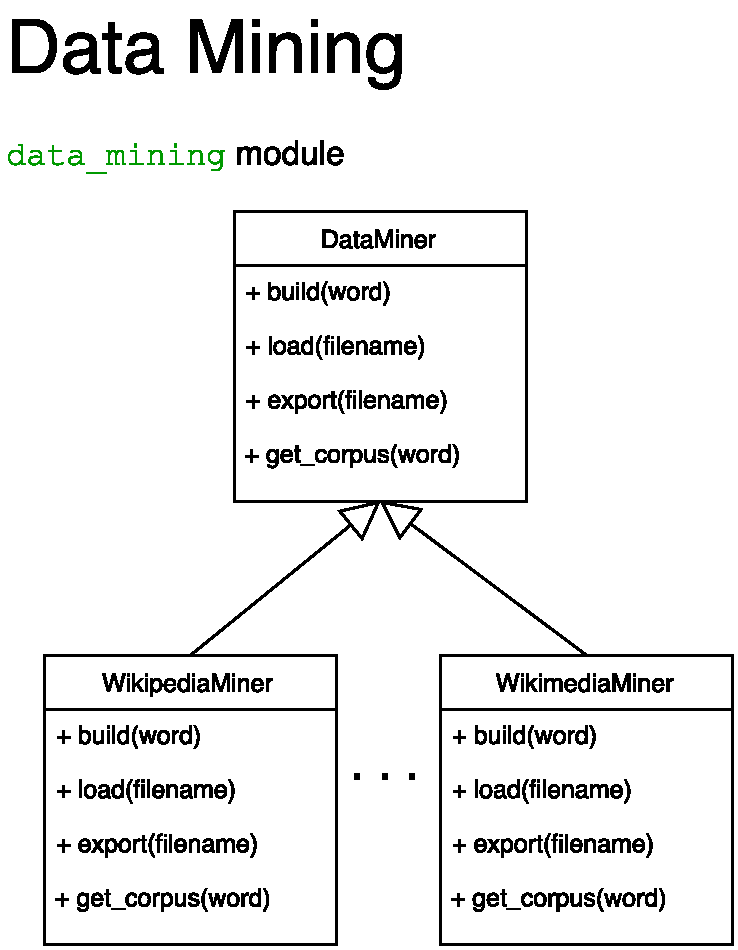
\includegraphics[width=12cm]{diagrams/Ambiruptor_data_mining.pdf}
    \caption{UML Diagram of data mining module}
    \label{fig:uml_data_mining}
\end{figure}

\begin{figure}[h!]
    \centering
    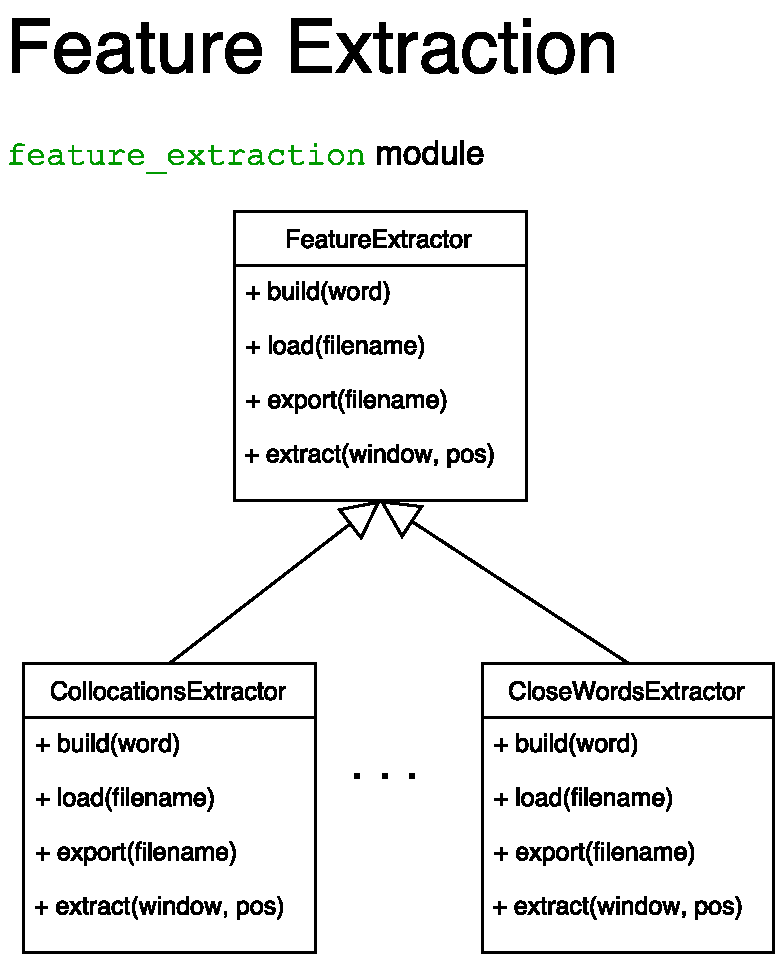
\includegraphics[width=12cm]{diagrams/Ambiruptor_feature_extraction.pdf}
    \caption{UML Diagram of feature extraction}
    \label{fig:uml_feature_extraction}
\end{figure}

\begin{figure}[h!]
    \centering
    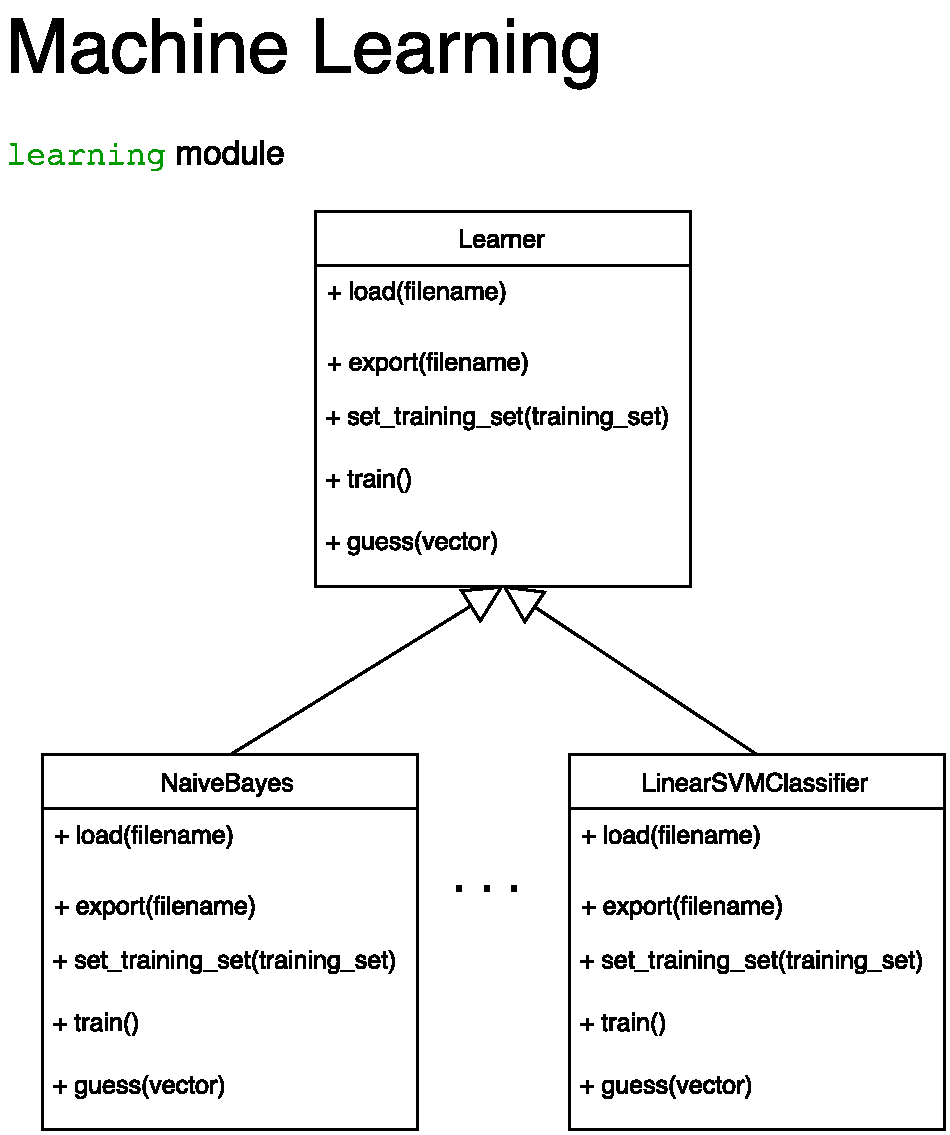
\includegraphics[width=12cm]{diagrams/Ambiruptor_learning.pdf}
    \caption{UML Diagram of learning module}
    \label{fig:uml_learning}
\end{figure}

\end{document}